%!TEX TS-program = pdflatex
%!TEX root = main.tex
%!TEX encoding = UTF-8 Unicode

\section{Infrastruttura di supporto}
%%\lstinputlisting[
%%firstline= 1,
%%lastline = 16
%%]{./code/covid19.mzn}
Per agevolare la raccolta dati e l'analisi delle soluzioni fornite dai due modelli ho sviluppato una piccola libreria python sfruttando i pacchetti \emph{minizinc} e \emph{clingo} che permettono di caricare, configurare e lanciare i rispettivi modelli.
Inoltre, ho implementato un visualizzatore delle soluzioni con \emph{ncurses} in python per potere valutare manualmente e confrontare meglio le soluzioni, questo è risultato molto utile per trovare errori durante la fase di modellazione.

\noindent
%\subsection{La libreria}
I file che permettono l'esecuzione dei modelli e salvano i loro output sono:
\begin{itemize}
  \item \emph{input\_generator.py} genera le istanze e le salva nei formati \emph{.lp} e \emph{.dzn} nelle relative cartelle \emph{inputs\_mzn} ed \emph{inputs\_lp}.
    Per fare ciò si appoggia a \emph{my\_lib.py}, istanziando la classe \emph{InputGenerator} e passando gli argomenti per gli intervalli di $H$ e $K$.
    Gli input vengono creati in modo casuale considerando il numero massimo di posti disponibili e poi saturandolo fino ad un livello casuale.
    In questo modo è possibile generare input difficili (molti ospiti ``scomodi'') oppure facili (se il numero di ospiti è basso rispetto al numero di posti).

  \item \emph{run.py} avvia l'esecuzione di entrambi i modelli su tutti gli input generati, salva gli output man mano che vengono trovate le soluzioni.
    Anche questo file si appoggia a \emph{my\_lib.py}, in particolare usa le classi \emph{RunnerMzn} e \emph{RunnerLp} che permettono di caricare i modelli indicati e di utilizzare le configurazioni migliori per ciascuno.
    Una barra di progresso indica la percentuale di input elaborati;

  \item \emph{run\_mzn.py} e \emph{run\_lp.py} permettono di eseguire un particolare modello su un input, specificandolo con il numero relativo. Ad es. \lstinline{python run_mzn.py 10} tornerà un \emph{pretty print} della soluzione dell'istanza \emph{inputs\_mzn/input\_10.dzn};

  \item \emph{my\_gloabals.py} contiene tutte le globali utili, come ad esempio il tempo di timeout per le esecuzioni dei modelli, oppure nomi di cartelle e file;

  \item \emph{batch\_saver.py} è risultato utile in fase di sviluppo dei modelli perché crea una copia di input, output e modelli in una cartella apposita.
  In questo modo è stato possibile confrontare le prestazioni di modelli diversi.
  Anche questo file si appoggia a \emph{my\_lib.py} ed utilizza la classe \emph{BatchCoordinator};

  \item \emph{my\_lib.py} contiene un insieme di classi che permettono di astrarre modelli, istanze, soluzioni oppure semplificare la creazione e gestione dei file.
\end{itemize}
Eseguendo \lstinline{python run.py} verranno create due cartelle, una per modello, contenenti i file \emph{.json} delle soluzioni, è qui riportato un esempio di una soluzione generata in questo modo.
\begin{lstlisting}
{
 "model_type": "MZN", "sat": true, "obj": 1,      
 "timeouted": false, "solveTime": 0.000832, "time": 0.09,
 "sol": {
    "K": 1, "H": 3,
    "M": [ 0 ],
    "P": [ 2, 2, 4, 4 ],
    "O": [ 1 ],
    "Q": [ 3, 5, 5 ]
 }
}
\end{lstlisting}
Infine, eseguendo il file \emph{in\_out\_visualizer.py} è possibile scorrere tra le soluzioni prodotte dai due modelli.
In \autoref{fig:esempio_2} si può osservare il programma in esecuzione:
a sinistra si ha la soluzione di Minizinc con rappresentazione grafica di camere e dei posti occupati;
a destra il modello ASP non ha generato alcuna soluzione perché è andato in timeout;
in basso si hanno informazioni riguardo all'input di partenza.
Il visualizzatore permette di scorrere avanti ed indietro tra le soluzioni contenute nelle cartelle \emph{outputs\_mzn} ed \emph{outputs\_lp}.
\begin{figure}[ht]
  \centering
  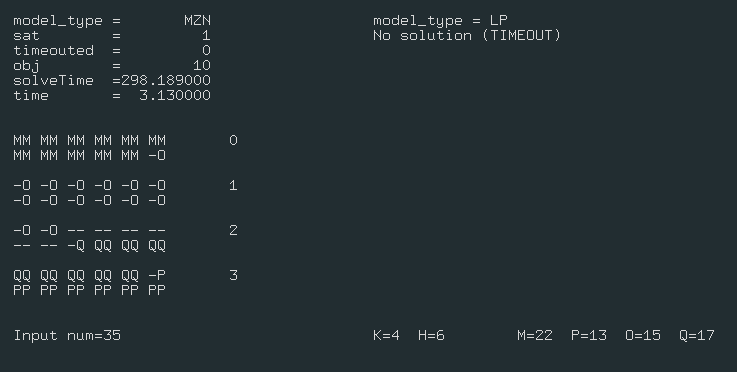
\includegraphics[width=.8\textwidth]{esempio_2}
  \caption{Schermata di \emph{in\_out\_visualizer.py}}
  \label{fig:esempio_2}
\end{figure}

